\section{Setting Up Program Options}\label{programOptions}

The first thing you'll want to do is set up your Program Options. Some
settings are required for features of Blue to work (i.e. Render
Settings, the Csound Documentation Root for opening opcode help), others
are there to help setup your project defaults and save you time when
creating new projects.

To open up the Program Options dialog, go to the File menu and click on
"Program Options".

Program Options - General

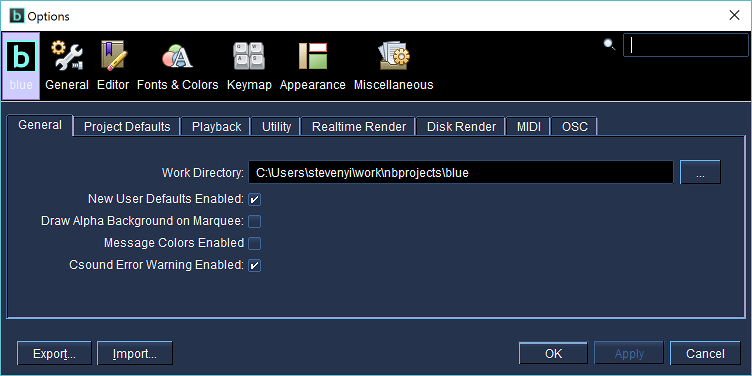
\includegraphics[width=1.00000\textwidth]{images/programOptions_general.png}

\begin{description}
\item[Csound Documentation Root]
This is the url of the root of your Csound Documentation. Blue uses this
for opening up Csound Documentation as well as when opening up help for
an opcode. The Csound Documentation Root can be local (i.e.
"file:///home/user/blue/manual/" or "file://c:/Programs and
Files/blue/manual/") or online (i.e.
"http://www.csounds.com/manual/html/").

You can get the Csound html documentation from
\href{http://www.csounds.com/manual}{} .
\item[Work Directory]
The default directory that Blue should open when loading/saving Blue
project files.
\item[Maintain Last Window State]
Enables saving of window location and size. If enabled, upon starting of
program, window states will be restored.
\item[New User Defaults Enabled]
Enables default text for different objects in Blue. Curently this
affects:

\begin{itemize}
\item
  CodeRepository - when adding new Code Snippet
\end{itemize}
\item[Draw Flat SoundObject Borders]
Enables older flat drawing style of SoundObject borders on the score
timeline.
\item[Draw Alpha Background on Marquee]
If this is enabled, when selecting a group of SoundObjects on the Score
Timeline the marquee that is drawn to show the selection area will paint
with an alpha-transparent white background. (May slow down performance
when enabled.)
\item[Show Csound Output]
If this is enabled, output from rendering with Csound will be shown in
the Csound Output Dialog (accessible from the Window menu or available
with the F7 shortcut). If disabled, output will be shown in the std.out
of the console that opens when Blue starts. (If the Blue starter script
has been modified not to show the console by using javaw instead of
java, then the output will not be able to be seen). It is recommended to
enable this option.
\item[Message Colors Enabled]
Since Csound5, the default for printed messages is to show them with
colors by using ANSI text modifiers. However, this only works within
ANSI-compliant consoles, and does not work within Blue's Csound Output
Dialog. It is recommended to keep this disabled if the "Show Csound
Output" option is enabled.
\item[Language]
Which language to use for Blue. This affects the labels of the User
Interface, messages given to the user in dialog boxes, menu titles, etc.
(Translation files may not always be up to of date so some UI items may
not be translated when not in English.)
\end{description}

Program Options - Project Defaults

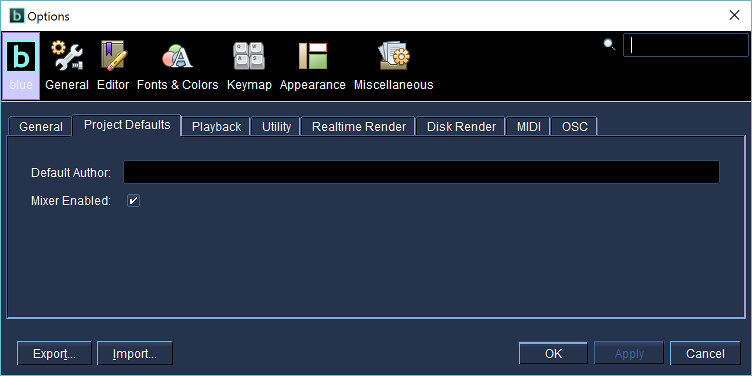
\includegraphics[width=1.00000\textwidth]{images/programOptions_projectDefaults.png}

These settings are used whenever new projects are created as defaults
for the project, unless a default.blue file is found in the user's Blue
home directory, in which case the settings from the default.blue file
are used.

\begin{description}
\item[Author]
Default author to use in new projects.
\item[Mixer Enabled]
Enable using the Blue Mixer in new projects by default.
\end{description}

Program Options - Playback

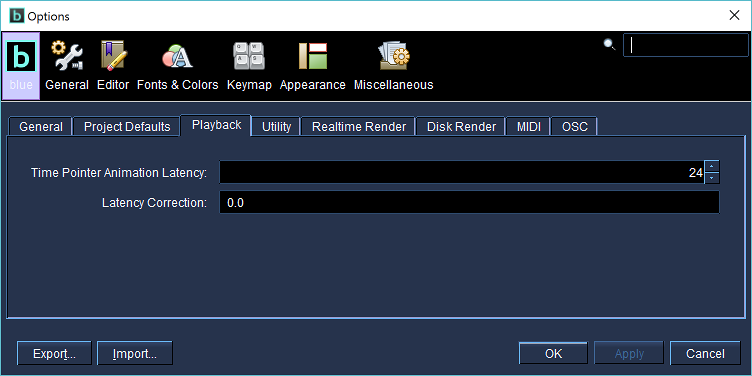
\includegraphics[width=1.00000\textwidth]{images/programOptions_playBack.png}

\begin{description}
\item[Time Pointer Animation Rate]
Rate of animation for time pointer to update when playing back in
realtime, expressed in frames per second. For example, the default value
of 20 means the time pointer is updated 20 times per second, giving a
smooth animation rate. Slower values may be desirable on slower
computers if the playback pointer is affecting performance.
\item[Latency Correction]
Float value in seconds to use as a correction for audio latency in the
user's sound playback mechanism. For example, if latency is quite bad on
your soundcard and there is a delay of .5 seconds between when audio is
passed to your soundcard and when the audio is actually realized from
the DAC, the visual time pointer for Blue may appear ahead in time of
what is being heard. Using a .5 value for latency correction would
correct for this.
\end{description}

Program Options - Utility

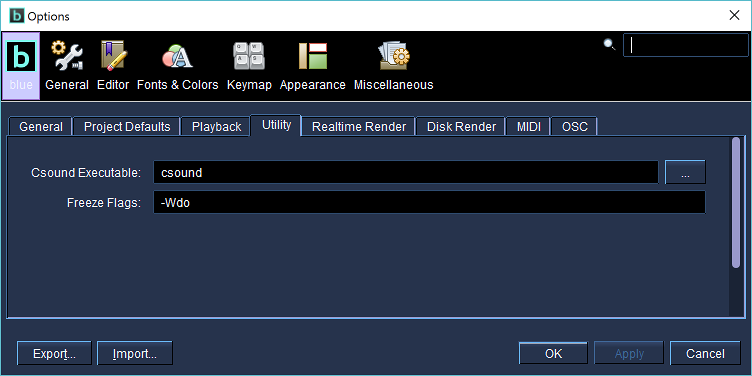
\includegraphics[width=1.00000\textwidth]{images/programOptions_utility.png}

\begin{description}
\item[Csound Executable]
This is the command for what version of Csound to execute when Blue uses
utilities that depend on Csound (for example, freezing SoundObjects, the
SoundFont Viewer utility). The default value of "csound" works if you
have a version of Csound in your path named "csound". You may use any
command here that would call Csound that would work as if you were
running csound from a terminal.

\begin{quote}
\textbf{Note}

The value defined for Csound Executable should only be the command to
call Csound and no other flags should be added here.
\end{quote}
\item[Freeze Flags]
These are the flags for Csound that Blue uses when performing
SoundObject freezing. Defaults are "-Ado" for Mac and "-Wdo" for all
other operating systems. Users may wish to modify this value if they
would their frozen soundObjects to be in a different format, i.e. 32-bit
float soundfiles.
\end{description}

Program Options - Realtime

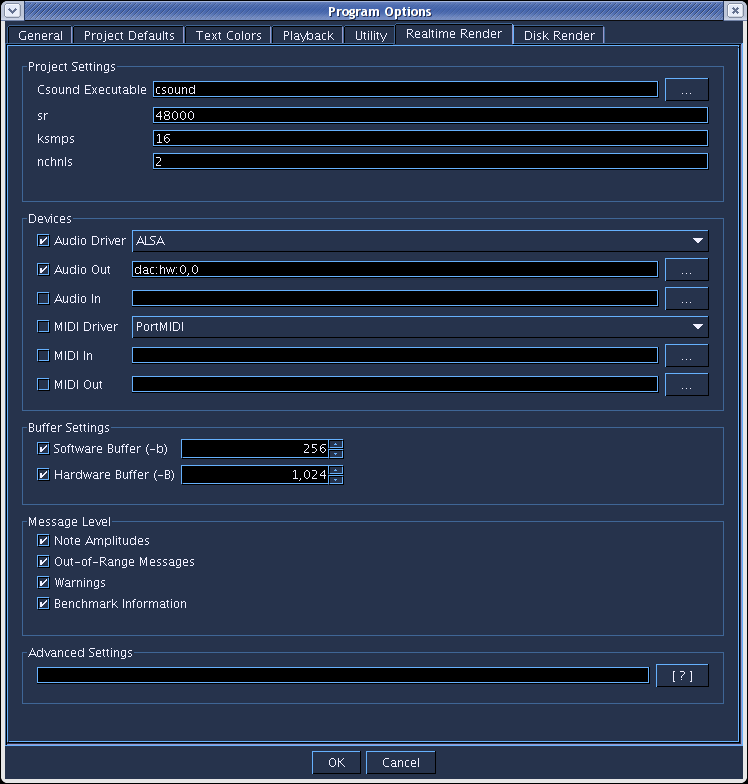
\includegraphics[width=1.00000\textwidth]{images/programOptions_realtime.png}

\begin{description}
\item[Csound Executable]
This is a command for what version of Csound to execute when Blue
renders the project in realtime. The default value of "csound" works if
you have a version of Csound in your path named "csound". You may use
any command here that would call csound that would work as if you were
running csound from a terminal.

Using the button marked "..." on the right will open up a file dialog so
that you can find and select the Csound executable to use to run Csound.

If you are using the API, you still need to have something set here. You
can set it to "csound" in that case.

\begin{quote}
\textbf{Note}

The value defined for Csound Executable should only be the command to
call Csound and no other flags should be added here.
\end{quote}
\item[Render Method]
Choose which render service to use for rendering the project. When the
program loads, Blue will first try to see if the Csound 6 API is
available and if so, show that option here. If it can not find the
Csound 6 API, it will search for the Csound 5 API and show that option
here instead if it is found. If neither is found, the Commandline Runner
option will always be available to use.

Note: If you have both Csound 5 and Csound 6 installed, you can force
Blue to ignore Csound 6 on load by adding "-J-DDISABLE\_CSOUND=true" to
the blue/etc/blue.conf file in the default\_options section. On OSX,
this will be in blue.app/Contents/Resources/blue/etc/blue.conf.
\item[sr]
Default sr to use for realtime settings in new projects.
\item[ksmps]
Default ksmps to use for realtime settings in new projects.
\item[0dbfs]
Default value to use for 0dbfs. Also, the checkbox denotes whether
projects should use 0dbfs by default or not.
\end{description}

\begin{description}
\item[Audio Driver]
Driver to use for audio input and output. This is equivalent to using
the -\/-rtaudio= flag setting on the commandline.

Enabling the checkbox determines if this value will be used at all when
rendering, and if so, will use the value from the dropdown as the driver
setting.
\item[Audio Out]
Audio output device to use. Equivalent to using -o flag setting on the
commandline. This setting is dependent on the setting used on the audio
driver setting. Using a value of "dac" will use the default device for
the driver.

The value of this setting will be used for all projects that set "Audio
Out" enabled in the project-level realtime render settings.

By selecting the {[}...{]} button to the right of this field, Blue will
try to detect what devices are available for the chosen Audio Driver. If
Blue is able to find the devices, a popup dialog will appear with a list
of available devices. Selecting from the popup will then populate the
textfield with the correct device string that Csound will use to choose
the device requested.

\begin{quote}
\textbf{Note}

If the driver is chosen but not enabled for use via its checkbox, when
auto-detecting, Blue will check for devices against the default driver
and not necessarily what is in the dropdown. Please be sure that if you
are planning to use the auto-detect feature with a particular driver
that you also select the driver and enable it with the checkbox.
\end{quote}

Enabling the checkbox determines if this device will be enabled by
default for new projects.
\item[Audio In]
Audio input device to use. Equivalent to using -i flag setting on the
commandline. This setting is dependent on the setting used on the audio
driver setting. Using a value of "adc" will use the default device for
the driver.

The value of this setting will be used for all projects that set "Audio
In" enabled in the project-level realtime render settings.

By selecting the {[}...{]} button to the right of this field, Blue will
try to detect what devices are available for the chosen Audio Driver. If
Blue is able to find the devices, a popup dialog will appear with a list
of available devices. Selecting from the popup will then populate the
textfield with the correct device string that Csound will use to choose
the device requested.

\begin{quote}
\textbf{Note}

If the driver is chosen but not enabled for use via its checkbox, when
auto-detecting, Blue will check for devices against the default driver
and not necessarily what is in the dropdown. Please be sure that if you
are planning to use the auto-detect feature with a particular driver
that you also select the driver and enable it with the checkbox.
\end{quote}

Enabling the checkbox determines if this device will be enabled by
default for new projects.
\item[MIDI Driver]
Driver to use for MIDI input and output. This is equivalent to using the
-\/-rtmidi= flag setting on the commandline.

Enabling the checkbox determines if this value will be used at all when
rendering, and if so, will use the value from the dropdown as the driver
setting.
\item[MIDI Out]
MIDI output device to use. Equivalent to using -Q flag setting on the
commandline. This setting is dependent on the setting used on the MIDI
driver setting.

The value of this setting will be used for all projects that set "MIDI
Out" enabled in the project-level realtime render settings.

By selecting the {[}...{]} button to the right of this field, Blue will
try to detect what devices are available for the chosen MIDI Driver. If
Blue is able to find the devices, a popup dialog will appear with a list
of available devices. Selecting from the popup will then populate the
textfield with the correct device string that Csound will use to choose
the device requested.

\begin{quote}
\textbf{Note}

If the driver is chosen but not enabled for use via its checkbox, when
auto-detecting, Blue will check for devices against the default driver
and not necessarily what is in the dropdown. Please be sure that if you
are planning to use the auto-detect feature with a particular driver
that you also select the driver and enable it with the checkbox.
\end{quote}

Enabling the checkbox determines if this device will be enabled by
default for new projects.
\item[MIDI In]
MIDI input device to use. Equivalent to using -M flag setting on the
commandline. This setting is dependent on the setting used on the audio
driver setting.

The value of this setting will be used for all projects that set "MIDI
In" enabled in the project-level realtime render settings.

By selecting the {[}...{]} button to the right of this field, Blue will
try to detect what devices are available for the chosen MIDI Driver. If
Blue is able to find the devices, a popup dialog will appear with a list
of available devices. Selecting from the popup will then populate the
textfield with the correct device string that Csound will use to choose
the device requested.

\begin{quote}
\textbf{Note}

If the driver is chosen but not enabled for use via its checkbox, when
auto-detecting, Blue will check for devices against the default driver
and not necessarily what is in the dropdown. Please be sure that if you
are planning to use the auto-detect feature with a particular driver
that you also select the driver and enable it with the checkbox.
\end{quote}

Enabling the checkbox determines if this device will be enabled by
default for new projects.
\end{description}

\begin{description}
\item[Software Buffer]
Size of software sample buffer to use (-b). For more information, see
CommandFlags section of Csound manual for settings.

Enabling the checkbox determines if this value will be used at all when
rendering.
\item[Hardware Buffer]
Size of hardware sample buffer to use (-B). For more information, see
CommandFlags section of Csound manual for settings.

Enabling the checkbox determines if this value will be used at all when
rendering.
\end{description}

\begin{description}
\item[Note Amplitudes]
Enables note amplitude messages from Csound (-m1)
\item[Out-of-Range Messages]
Enables samples out of range messages from Csound (-m2)
\item[Warnings]
Enables warning messages from Csound (-m4)
\item[Benchmark Information]
Enables benchmark information from Csound (-m128)
\end{description}

\begin{description}
\item[Advanced Settings]
Extra flags to append to the commandline that might not be covered by
options in the UI. Pressing the {[}?{]} button will open the
documentation for the Csound command flags (Csound Documentation Root
but be set for this to work).
\end{description}

Program Options - Disk Render

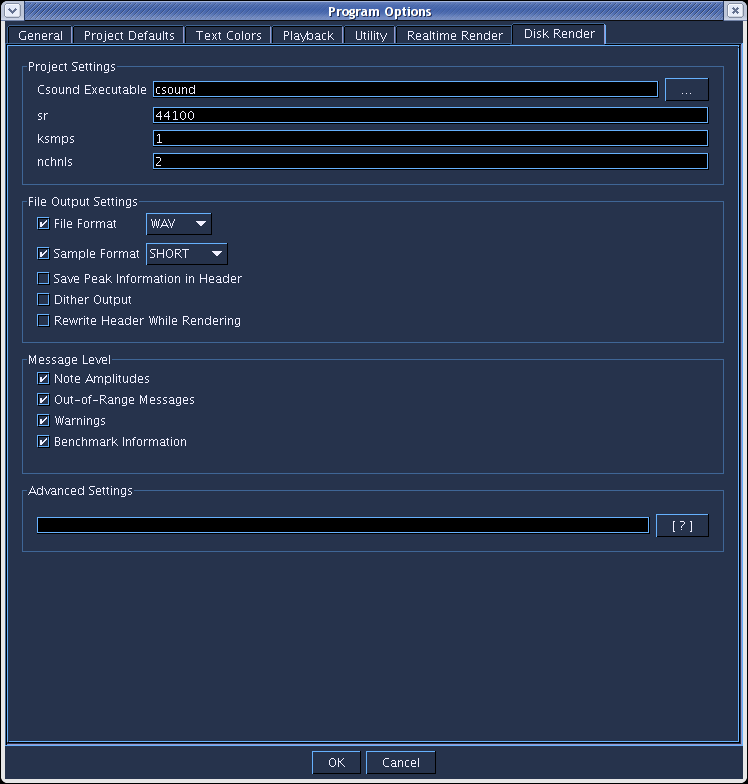
\includegraphics[width=1.00000\textwidth]{images/programOptions_diskRender.png}

\begin{description}
\item[Csound Executable]
This is a command for what version of csound to execute when Blue
renders the project to disk. The default value of "csound" works if you
have a version of Csound in your path named "csound". You may use any
command here that would call csound that would work as if you were
running csound from a terminal.

Using the button marked "..." on the right will open up a file dialog so
that you can find and select the csound executable to use to run Csound.

\begin{quote}
\textbf{Note}

The value defined for Csound Executable should only be the command to
call Csound and no other flags should be added here.
\end{quote}
\item[Render Method]
Choose which render service to use for rendering the project. When the
program loads, Blue will first try to see if the Csound 6 API is
available and if so, show that option here. If it can not find the
Csound 6 API, it will search for the Csound 5 API and show that option
here instead if it is found. If neither is found, the Commandline Runner
option will always be available to use.

Note: If you have both Csound 5 and Csound 6 installed, you can force
Blue to ignore Csound 6 on load by adding "-J-DDISABLE\_CSOUND=true" to
the blue/etc/blue.conf file in the default\_options section. On OSX,
this will be in blue.app/Contents/Resources/blue/etc/blue.conf.
\item[sr]
Default sr to use for disk render settings in new projects.
\item[ksmps]
Default ksmps to use for disk render settings in new projects.
\item[nchnls]
Default nchnls to use for disk render settings in new projects.
\item[0dbfs]
Default value to use for 0dbfs. Also, the checkbox denotes whether
projects should use 0dbfs by default or not.
\end{description}

\begin{description}
\item[Enabled]
Enable using custom play command when using "Render and Play". If not
enabled, Blue's built-in audio player will be used once the project is
finished rendering to disk.
\item[Command]
Command to call after finished rendering a project. The command line
given should use the \$outfile property where the name of the generated
audio file should be passed to the program. For example, to open the
rendered audio with VLC on Mac OSX, you can use this command line:

\begin{verbatim}
open -a VLC $outfile
\end{verbatim}
\end{description}

\begin{description}
\item[File Format]
File format to use (i.e. WAV, AIFF, AU, etc.)

Enabling the checkbox determines if this value will be used at all when
rendering.
\item[Sample Format]
Sample format to use. The default of SHORT is the same as 16-bit integer
audio (the same as used for CD's). Other formats are available in the
dropdown to use.

Enabling the checkbox determines if this value will be used at all when
rendering.
\item[Save Peak Information in Header]
Save the peak information in the file header.

Enabling the checkbox determines if this value will be used at all when
rendering.
\item[Dither Output]
Use dither on output.

Enabling the checkbox determines if this value will be used at all when
rendering.
\item[Rewrite Header while Rendering]
Rewrite the file header while rendering. This makes it possible to play
the audio file in the middle of a render and is useful when the
rendering of the project will take a very long time. However, it does
slow down overall render time.

Enabling the checkbox determines if this value will be used at all when
rendering.
\end{description}

\begin{description}
\item[Note Amplitudes]
Enables note amplitude messages from Csound (-m1)
\item[Out-of-Range Messages]
Enables samples out of range messages from Csound (-m2)
\item[Warnings]
Enables warning messages from Csound (-m4)
\item[Benchmark Information]
Enables benchmark information from Csound (-m128)
\end{description}

\begin{description}
\item[Advanced Settings]
Extra flags to append to the commandline that might not be covered by
options in the UI. Pressing the {[}?{]} button will open the
documentation for the Csound command flags (Csound Documentation Root
but be set for this to work).
\end{description}

Program Options - Disk Render

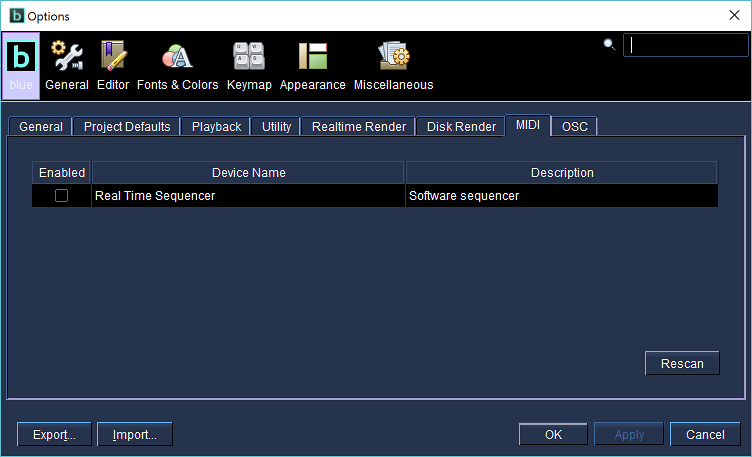
\includegraphics{images/programOptions_midi.png}

These settings are for Blue's MIDI input, used with
\protect\hyperlink{blueLive}{BlueLive}. The table shows what devices are
currently available, and whether they are enabled for use with BlueLive
or not. You can use the "rescan" button to search for devices if you
have just plugged in a device.

Program Options - OSC

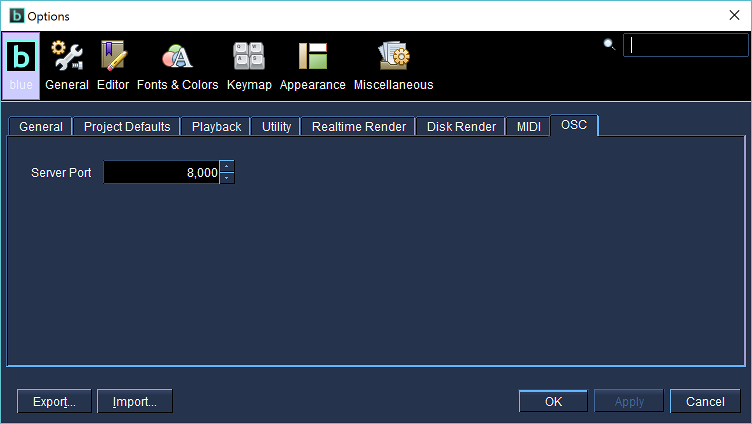
\includegraphics{images/programOptions_osc.png}

This allows you to set what port Blue will listen to for incoming OSC
messages. Defaults to 8000. The following messages are understood by
Blue:

\begin{itemize}
\item
  /score/play
\item
  /score/stop
\item
  /score/rewind
\item
  /score/markerNext
\item
  /score/markerPrevious
\item
  /blueLive/onOff
\item
  /blueLive/recompile
\item
  /blueLive/allNotesOff
\item
  /blueLive/toggleMidiInput
\end{itemize}
